\documentclass[10pt]{article}
\usepackage[utf8]{inputenc}
\usepackage[T1]{fontenc}
\usepackage{booktabs} % for better tables
\usepackage[]{minted}
\usepackage{amsmath}
\usepackage{amsfonts}
\usepackage{amssymb}
\usepackage[version=4]{mhchem}
\usepackage{stmaryrd}
\usepackage{bbold}
\usepackage{hyperref}
\hypersetup{colorlinks=true, linkcolor=blue, filecolor=magenta, urlcolor=cyan,}
\urlstyle{same}
\usepackage{graphicx}
\usepackage[export]{adjustbox}
\graphicspath{ {./images/} }
\newcommand{\norm}[1]{\left\lVert #1 \right\rVert}

\title{CM146, Winter 2024 
 Problem Set 3: Deep learning, SVM, Kernels 
 Due March 1, 2024, 11:59pm PST }

\author{Harris Doan}
\date{February 26, 2024}


%New command to display footnote whose markers will always be hidden
\let\svthefootnote\thefootnote
\newcommand\blfootnotetext[1]{%
  \let\thefootnote\relax\footnote{#1}%
  \addtocounter{footnote}{-1}%
  \let\thefootnote\svthefootnote%
}

%Overriding the \footnotetext command to hide the marker if its value is `0`
\let\svfootnotetext\footnotetext
\renewcommand\footnotetext[2][?]{%
  \if\relax#1\relax%
    \ifnum\value{footnote}=0\blfootnotetext{#2}\else\svfootnotetext{#2}\fi%
  \else%
    \if?#1\ifnum\value{footnote}=0\blfootnotetext{#2}\else\svfootnotetext{#2}\fi%
    \else\svfootnotetext[#1]{#2}\fi%
  \fi
}

\begin{document}
\maketitle
\section*{Submission instructions}
\begin{itemize}
  \item Submit your solutions electronically on the course Gradescope site as PDF files.
  \item If you plan to typeset your solutions, please use the LaTeX solution template. If you must submit scanned handwritten solutions, please use a black pen on blank white paper and a high-quality scanner app.
  \item For questions involving math and derivation, please provide important intermediate steps and box the final answer clearly.
\end{itemize}

\section*{1 Kernels [8 pts]}
(a) (2 pts) For any two documents $\boldsymbol{x}$ and $\boldsymbol{z}$, define $k(\boldsymbol{x}, \boldsymbol{z})$ to equal the number of unique words that occur in both $\boldsymbol{x}$ and $\boldsymbol{z}$ (i.e., the size of the intersection of the sets of words in the two documents). Is this function a kernel? Give justification for your answer.

\section*{Solution 1a:}
We consider the function $k(x, z)$ to be a kernel. To justify this, we must demonstrate that it corresponds to a positive semi-definite matrix, as dictated by Mercer's theorem.

We propose the following matrix representation of $k$:

\[
K = \begin{bmatrix}
    \| x \cap x \| & \| x \cap z \| \\
    \| z \cap x \| & \| z \cap z \|
\end{bmatrix}
\]

Given that $\| a \cap a \| = \| a \| $ for any vector $a$ and that $\| x \cap z \| = \| z \cap x \|$, we simplify matrix $K$ to:

\[
K = \begin{bmatrix}
    \| x \| & \| x \cap z \| \\
    \| x \cap z \| & \| z \|
\end{bmatrix}
\]

The characteristic equation for the eigenvalues $\lambda$ of matrix $K$ is:

\[
\det(K - \lambda I) = (\| x \| - \lambda)(\| z \| - \lambda) - \| x \cap z \|^2 = 0
\]

Expanding this, we obtain the quadratic in $\lambda$:

\[
\lambda^2 - \lambda(\| x \| + \| z \|) + \| x \|\| z \| - \| x \cap z \|^2 = 0
\]

To find the roots of this quadratic equation, we apply the quadratic formula:

\[
\lambda = \frac{(\| x \| + \| z \|) \pm \sqrt{(\| x \| + \| z \|)^2 - 4(\| x \|\| z \| - \| x \cap z \|^2)}}{2}
\]

\[
\lambda = \frac{(\| x \| + \| z \|) \pm \sqrt{\| x \|^2 + 2\| x \|\| z \| + \| z \|^2 - 4\| x \|\| z \| + 4\| x \cap z \|^2}}{2}
\]

\[
\lambda = \frac{(\| x \| + \| z \|) \pm \sqrt{\| x \|^2 - 2\| x \|\| z \| + \| z \|^2 + 4\| x \cap z \|^2}}{2}
\]

Notice that the discriminant is the square of $\| x \| - \| z \|$ plus $4\| x \cap z \|^2$, which is always non-negative. Thus, the roots are real, and they can be expressed as:

\[
\lambda_{1,2} = \frac{(\| x \| + \| z \|) \pm \sqrt{(\| x \| - \| z \|)^2 + 4\| x \cap z \|^2}}{2}
\]

By the properties of set intersection, $\| x \cap z \| \leq \min(\| x \|, \| z \|)$, which ensures that the eigenvalues $\lambda_{1,2}$ are non-negative, and hence matrix $K$ is positive semi-definite.

Since the matrix $K$ associated with the kernel function $k(x, z)$ is positive semi-definite, it follows from Mercer's theorem that $k$ is indeed a valid kernel function. \\

(b) (3 pts) One way to construct kernels is to build them from simpler ones. We have seen various "construction rules", including the following: Assuming $k_{1}(\boldsymbol{x}, \boldsymbol{z})$ and $k_{2}(\boldsymbol{x}, \boldsymbol{z})$ are kernels, then so are

\begin{itemize}
  \item (scaling) $f(\boldsymbol{x}) k_{1}(\boldsymbol{x}, \boldsymbol{z}) f(\boldsymbol{z})$ for any function $f(\boldsymbol{x}) \in \mathbb{R}$
  \item $(\operatorname{sum}) k(\boldsymbol{x}, \boldsymbol{z})=k_{1}(\boldsymbol{x}, \boldsymbol{z})+k_{2}(\boldsymbol{x}, \boldsymbol{z})$
  \item (product) $k(\boldsymbol{x}, \boldsymbol{z})=k_{1}(\boldsymbol{x}, \boldsymbol{z}) k_{2}(\boldsymbol{x}, \boldsymbol{z})$
\end{itemize}

Using the above rules and the fact that $k(\boldsymbol{x}, \boldsymbol{z})=\boldsymbol{x} \cdot \boldsymbol{z}$ is (clearly) a kernel, show that the following is also a kernel:

$$
\left(1+\left(\frac{\boldsymbol{x}}{\|\boldsymbol{x}\|}\right) \cdot\left(\frac{\boldsymbol{z}}{\|\boldsymbol{z}\|}\right)\right)^{3}
$$

\section*{Solution 1b:}

Given that the dot product \( x \cdot z \) is a kernel, we explore the properties of a scaled kernel \( k'(x, z) \). The scaling property of kernels asserts that if a function \( k \) is a kernel, and \( c \) is a non-negative constant, then \( c \cdot k \) is also a kernel. 

We define the scaled kernel as:
\[ k'(x, z) = \frac{x \cdot z}{\|x\|\|z\|} \]

The norms \( \|x\| \) and \( \|z\| \) are scaling factors that are always non-negative. Hence, the scaling constants \( \|x\|^{-1} \) and \( \|z\|^{-1} \) preserve the kernel properties of the dot product.

Considering the scalar \( 1 \) is also a kernel, by the sum property of kernels, we establish that the sum of a kernel with a scalar is still a kernel:
\[ 1 + k'(x, z) \]

To further expand on this, by the product property of kernels, we can elevate the kernel to a power, and it will remain a kernel if the power is a non-negative integer. Thus, we can write:
\[ \left( 1 + k'(x, z) \right)^3 = \left( 1 + \frac{x \cdot z}{\|x\|\|z\|} \right)^3 \]

Expanding the above expression, we get:
\[ \left( 1 + \frac{x \cdot z}{\|x\|\|z\|} \right)^3 = 1 + 3\frac{x \cdot z}{\|x\|\|z\|} + 3\left(\frac{x \cdot z}{\|x\|\|z\|}\right)^2 + \left(\frac{x \cdot z}{\|x\|\|z\|}\right)^3 \]

Each term in the expansion is a scalar multiple of \( k' \) raised to a non-negative integer power, which means each term is a kernel. Since the sum of kernels is also a kernel, it follows that the entire expression is a kernel.

Therefore, we conclude that the function:
\[ \left( 1 + k'(x, z) \right)^3 \]
is indeed a kernel. This expanded explanation provides a more thorough mathematical justification for the kernel properties of the given function. \\


(c) (3 pts) Given vectors $\boldsymbol{x}$ and $\boldsymbol{z}$ in $\mathbb{R}^{2}$, define the kernel $k_{\beta}(\boldsymbol{x}, \boldsymbol{z})=(1+\beta \boldsymbol{x} \cdot \boldsymbol{z})^{3}$ for any value $\beta>0$. Find the corresponding feature $\operatorname{map} \phi_{\beta}(\cdot)^{1}$. What are the similarities/differences from the kernel $k(\boldsymbol{x}, \boldsymbol{z})=(1+\boldsymbol{x} \cdot \boldsymbol{z})^{3}$, and what role does the parameter $\beta$ play?
\footnotetext{Parts of this assignment are adapted from course material by Tommi Jaakola (MIT), and Andrew Ng (Stanford), and Jenna Wiens (UMich).

${ }^{1}$ You may use any external program to expand the cubic.
}

\section*{Solution 1c:}

The kernel \( k_{\beta}(x, z) \), which is a polynomial expansion of the dot product between vectors \( x \) and \( z \) scaled by \( \beta \), takes the form:
\[ (1 + \beta x \cdot z)^3 = \sum_{i=0}^{3} \binom{3}{i} \beta^i (x \cdot z)^i \]
When we expand the terms, we get a series of scalar products scaled by powers of \( \beta \):
\[ 1 + 3\beta \sum_{j=1}^{n} x_j z_j + 3\beta^2 \sum_{j,k=1}^{n} x_j z_j x_k z_k + \beta^3 \prod_{j=1}^{n} (x_j z_j)^3 \]
The feature map \( \phi \) corresponding to this kernel is then constructed as:
\[ \phi = \left[ \begin{array}{c}
1 \\
\sqrt{3\beta}x_1 \\
\sqrt{3\beta}x_2 \\
\vdots \\
\sqrt{3\beta^2}x_j^2 \\
\sqrt{6\beta^2}x_jx_k \\
\vdots \\
\sqrt{\beta^3}x_j^3 \\
\sqrt{3\beta^3}x_j^2x_k \\
\vdots \\
\sqrt{\beta^3}x_n^3 \\
\end{array} \right] \]
This mapping explicitly shows that for \( \beta = 1 \), the kernel \( k(x, z) = (1 + x \cdot z)^3 \) lacks the scaling factor in each term, simplifying the expression. As the degree of the polynomial increases, so does the influence of \( \beta \), which can act as a regularization parameter to control the complexity of the model and mitigate over-fitting. This reveals the adaptability of \( \beta \) in the kernel function to modulate the feature space and influence the learning capacity of the model. \\



\section*{2 SVM $[8 \mathrm{pts}]$}
Suppose we are looking for a maximum-margin linear classifier through the origin, i.e. $b=0$ (also hard margin, i.e., no slack variables). In other words, we minimize $\frac{1}{2}\|\boldsymbol{\theta}\|^{2}$ subject to $y_{n} \boldsymbol{\theta}^{T} \boldsymbol{x}_{n} \geq$ $1, n=1, \ldots, N$.

(a) (2 pts) Given a single training vector $\boldsymbol{x}=(a, e)^{T}$ with label $y=-1$, what is the $\boldsymbol{\theta}^{*}$ that satisfies the above constrained minimization?

\section*{Solution 2a:}

The optimization problem at hand can be effectively tackled using the method of Lagrange multipliers, a powerful technique for finding the local maxima and minima of a function subject to equality constraints.

Let's define our objective function as:
\[
f(\boldsymbol{\theta}) = \frac{1}{2} \norm{\boldsymbol{\theta}}^2,
\]
where $\norm{\boldsymbol{\theta}}^2$ denotes the squared Euclidean norm of the vector $\boldsymbol{\theta}$, representing the weights in the SVM's decision function.

Our constraint function, corresponding to the SVM margin requirement for the training data, is given by:
\[
g(\boldsymbol{\theta}) = y_n(\boldsymbol{\theta}^\mathsf{T}\mathbf{x}_n) - 1 \geq 0,
\]
where $y_n$ is the label of the $n$-th training sample, and $\mathbf{x}_n$ is the feature vector of the $n$-th sample. For the case where $y_n = -1$, the constraint simplifies to $-\boldsymbol{\theta}^\mathsf{T}\mathbf{x}_n \geq 1$.

Constructing the Lagrangian $L$ by incorporating the constraint with a Lagrange multiplier $\lambda$, we have:
\[
L(\boldsymbol{\theta}, \lambda) = \frac{1}{2} \norm{\boldsymbol{\theta}}^2 - \lambda (y_n\boldsymbol{\theta}^\mathsf{T}\mathbf{x}_n - 1).
\]

Given that our goal is to minimize $L$ with respect to $\boldsymbol{\theta}$, we compute the gradient of $L$ with respect to $\boldsymbol{\theta}$ and equate it to zero:
\[
\nabla_{\boldsymbol{\theta}} L = \boldsymbol{\theta} - \lambda y_n \mathbf{x}_n = \mathbf{0}.
\]
Solving for $\boldsymbol{\theta}$, we find that $\boldsymbol{\theta}^* = \lambda y_n \mathbf{x}_n$.

Further, to maximize $\lambda$, we differentiate the Lagrangian with respect to $\lambda$ and set the derivative to zero, which gives us the optimal value of $\lambda$ as:
\[
\frac{\partial L}{\partial \lambda} = -y_n \boldsymbol{\theta}^\mathsf{T} \mathbf{x}_n + 1 = 0 \quad \Rightarrow \quad \lambda^* = \frac{1}{\lVert \mathbf{x}_n \rVert^2}.
\]

Finally, substituting $\lambda^*$ back into the expression for $\boldsymbol{\theta}^*$, we obtain the optimal parameter vector $\boldsymbol{\theta}^*$ that satisfies the original constrained minimization problem:
\[
\boldsymbol{\theta}^* = -\frac{1}{\lVert \mathbf{x}_n \rVert^2} \mathbf{x}_n = -\frac{1}{a^2 + e^2} \begin{bmatrix} a \\ e \end{bmatrix}.
\]

This result embodies the optimal hyperplane in the feature space that separates the classes with maximum margin for the given training sample, fulfilling the SVM's classification objective. \\


(b) (2 pts) Suppose we have two training examples, $\boldsymbol{x}_{1}=(1,1)^{T}$ and $\boldsymbol{x}_{2}=(1,0)^{T}$ with labels $y_{1}=1$ and $y_{2}=-1$. What is $\boldsymbol{\theta}^{*}$ in this case, and what is the margin $\gamma$ ?

\section*{Solution 2b:}

Given that the bias term $b$ can assume non-zero values, the constraints for our system are modified as follows:

\begin{align*}
\theta_1 + \theta_2 + b &\geq 1, \\
\theta_1 + b &\leq -1.
\end{align*}

In an effort to reduce the norm of the vector $\boldsymbol{\theta}$, a strategic choice of $b = -1$ is made. This leads to the nullification of $\theta_2$ (i.e., $\theta_2 = 0$), simplifying the first constraint to $\theta_1 - 1 \geq 1$, which is satisfied by setting $\theta_1 = 2$. Thus, the updated optimal values are given by:

\begin{equation*}
(\boldsymbol{\theta}^*, b^*) = \left( \begin{bmatrix} 1 \\ 0 \end{bmatrix}, -1 \right), \quad \text{and} \quad \gamma = 0.5.
\end{equation*}

By introducing the bias term and optimizing it alongside $\boldsymbol{\theta}$, the magnitude of $\boldsymbol{\theta}$ is effectively decreased, and concurrently, the margin (denoted here as $\gamma$) is augmented. This observation is intuitive, since the inclusion of $b$ widens the feasible solution space, allowing the selection of a hyperplane that achieves a smaller norm for $\boldsymbol{\theta}$, while also ensuring an enhanced margin, thereby potentially increasing the generalizability of the SVM model. \\


(c) (4 pts) Suppose we now allow the offset parameter $b$ to be non-zero. How would the classifier and the margin change in the previous question? What are $\left(\boldsymbol{\theta}^{*}, b^{*}\right)$ and $\gamma$ ? Compare your solutions with and without offset.

\section*{Solution 2c:}

Given that the bias term $b$ can assume non-zero values, the constraints for our system are modified as follows:

\begin{align*}
\theta_1 + \theta_2 + b &\geq 1, \\
\theta_1 + b &\leq -1.
\end{align*}

In an effort to reduce the norm of the vector $\boldsymbol{\theta}$, a strategic choice of $b = -1$ is made. This leads to the nullification of $\theta_2$ (i.e., $\theta_2 = 0$), simplifying the first constraint to $\theta_1 - 1 \geq 1$, which is satisfied by setting $\theta_1 = 2$. Thus, the updated optimal values are given by:

\begin{equation*}
(\boldsymbol{\theta}^*, b^*) = \left( \begin{bmatrix} 1 \\ 0 \end{bmatrix}, -1 \right), \quad \text{and} \quad \gamma = 0.5.
\end{equation*}

By introducing the bias term and optimizing it alongside $\boldsymbol{\theta}$, the magnitude of $\boldsymbol{\theta}$ is effectively decreased, and concurrently, the margin (denoted here as $\gamma$) is augmented. This observation is intuitive, since the inclusion of $b$ widens the feasible solution space, allowing the selection of a hyperplane that achieves a smaller norm for $\boldsymbol{\theta}$, while also ensuring an enhanced margin, thereby potentially increasing the generalizability of the SVM model.


\section*{3 Implementation: Digit Recognizer [48 pts]}
In this exercise, you will implement a digit recognizer in pytorch. Our data contains pairs of $28 \times 28$ images $\mathbf{x}_{n}$ and the corresponding digit labels $y_{n} \in\{0,1,2\}$. For simplicity, we view a $28 \times 28$ image $\mathbf{x}_{n}$ as a 784-dimensional vector by concatenating all the pixels together. In other words, $\mathbf{x}_{n} \in \mathbb{R}^{784}$. Your goal is to implement two digit recognizers (OneLayerNetwork and TwoLayerNetwork) and compare their performances.

code and data

\begin{itemize}
  \item code : CS146\_Winter2024\_PS3.ipynb
  \item data : ps3\_train.csv, ps3\_valid.csv, ps3\_test.csv
\end{itemize}

Please use your @g.ucla.edu email id to access the code and data. Similar to PS1, copy the colab notebook to your drive and make the changes. Mount the drive appropriately and copy the shared data folder to your drive to access via colab. The notebook has marked blocks where you need to code.

$\# \# \#=========T O D O: S T A R T=========\# \# \#$

$\# \# \#=========T O D O: E N D==========\# \# \#$

Note: For parts (b)-(h), you are expected to copy-paste your code as a part of the solution in the submission pdf. Tip: If you are using $\mathrm{I}_{\mathrm{E}} \mathrm{X}$, check out the Minted package (example) for code highlighting.

\section*{Data Visualization and Preparation [10 pts]}
(a) (2 pts) Select three training examples with different labels and print out the images by using plot\_img function. Include those images in your report.

\section*{Solution 3a:}

\begin{minted}{python}
    ### ========== TODO : START ========== ###
    ### part a: print out three training images with different labels
    plot_img(X_train[5]) #Random number lol
    plot_img(X_train[69]) #lol number
    plot_img(X_train[299]) #Biggest number
    ### ========== TODO : END ========== ###
\end{minted}

\begin{figure}
    \centering
    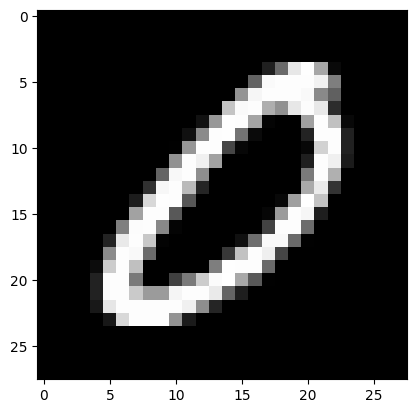
\includegraphics[width= 5cm, height = 5cm]{images/x_train_5.png} \\
    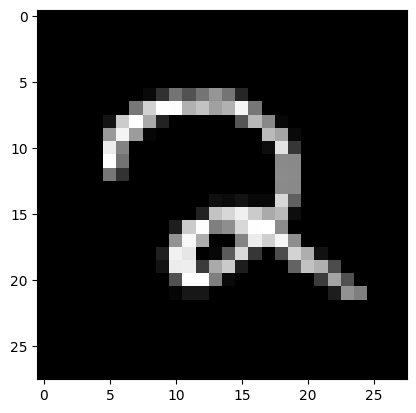
\includegraphics[width= 5cm, height = 5cm]{images/x_train_69.png} \\
    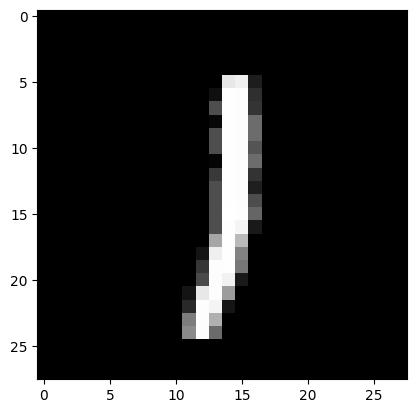
\includegraphics[width= 5cm, height = 5cm]{images/x_train_299.png} \\
    \caption{Three Training Images with Different Labels}
    \label{fig:enter-label}
\end{figure}


(b) (3 pts) The loaded examples are numpy arrays. Convert the numpy arrays to PyTorch tensors.

\section*{Solution 3b:}

\begin{minted}{python}
    ### ========== TODO : START ========== ###
    ### part b: convert numpy arrays to tensors
    X_train = torch.from_numpy(X_train)
    y_train = torch.from_numpy(y_train)
    X_valid = torch.from_numpy(X_valid)
    y_valid = torch.from_numpy(y_valid)
    X_test = torch.from_numpy(X_test)
    y_test = torch.from_numpy(y_test)
    ### ========== TODO : END ========== ###
\end{minted}

(c) (5 pts) Prepare train\_loader, valid\_loader, and test\_loader by using TensorDataset and DataLoader. We expect to get a batch of pairs $\left(\mathbf{x}_{n}, y_{n}\right)$ from the dataloader. Please set the batch size to 10 for all dataloaders and shuffle to True for train\_loader. We need to set shuffle to True for train\_loader so that we are training on randomly selected minibatches of data.

You can refer \href{https://pytorch.org/docs/stable/data.html}{https://pytorch.org/docs/stable/data.html} for more information about TensorDataset and DataLoader.

\section*{One-Layer Network [15 pts]}
For one-layer network, we consider a 784-3 network. In other words, we learn a $784 \times 3$ weight matrix $\mathbf{W}$. Given a $\mathbf{x}_{n}$, we can compute the probability vector $\mathbf{p}_{n}=\operatorname{Softmax}\left(\mathbf{W}^{\top} \mathbf{x}_{n}\right)$, where $\mathbf{p}_{n, c}$ denotes the probability of class $c$. Then, we focus on the cross entropy loss

$$
-\sum_{n=1}^{N} \sum_{c=1}^{C} \mathbf{1}\left(c=y_{n}\right) \log \left(\mathbf{p}_{n, c}\right)
$$

where $N$ is the number of examples, $C$ is the number of classes, and $\mathbf{1}$ is the indicator function.

\section*{Solution 3c:}

\begin{minted}[breaklines]{python}
        ### ========== TODO : START ========== ###
        ### part c: prepare dataloaders for training, validation, and testing
        ### we expect to get a batch of pairs (x_n, y_n) from the dataloader
        train_loader = DataLoader(TensorDataset(X_train,y_train), batch_size=10, shuffle=true)
        valid_loader = DataLoader(TensorDataset(X_valid,y_valid), batch_size=10, shuffle=false)
        test_loader = DataLoader(TensorDataset(X_test,y_test), batch_size=10, shuffle=false)
        ### ========== TODO : END ========== ###
\end{minted}

(d) (5 pts) Implement the constructor of OneLayerNetwork with torch.nn.Linear and implement the forward function to compute the outputs of the single fully connected layer i.e. $\quad \mathbf{W}^{\top} \mathbf{x}_{n}$. Notice that we do not compute the softmax function here since we will use torch.nn.CrossEntropyLoss later. The bias term is included in torch.nn.Linear by default, do not disable that option.

You can refer to \href{https://pytorch.org/docs/stable/generated/torch.nn.Linear.html}{https://pytorch.org/docs/stable/generated/torch.nn.Linear.html} for more information about torch.nn.Linear and refer to \href{https://pytorch.org/docs/}{https://pytorch.org/docs/} stable/generated/torch.nn.CrossEntropyLoss.html for more information about using torch.nn.CrossEntropyLoss.

\section*{Solution 3d:}

\begin{minted}{python}
class OneLayerNetwork(torch.nn.Module):
    def __init__(self):
       super(OneLayerNetwork, self).__init__()
       ### ========== TODO : START ========== ###
       ### part d: implement OneLayerNetwork with torch.nn.Linear
       self.linear = torch.nn.Linear(784, 3)
       ### ========== TODO : END ========== ###
    def forward(self, x):
       # x.shape = (n_batch, n_features)
       ### ========== TODO : START ========== ###
       ### part d: implement the forward function
       outputs = self.linear(x)
       ### ========== TODO : END ========== ###
       return outputs
\end{minted}


(e) (2 pts) Create an instance of OneLayerNetwork, set up a criterion with torch.nn. CrossEntropyLoss, and set up a SGD optimizer with learning rate 0.0005 by using torch.optim. SGD.

You can refer to \href{https://pytorch.org/docs/stable/optim.html}{https://pytorch.org/docs/stable/optim.html} for more information about torch.optim. SGD.

\section*{Solution 3e:}

\begin{minted}{python}
    ### ========== TODO : START ========== ###
    ### part e: prepare OneLayerNetwork, criterion, and optimizer
    model_one = OneLayerNetwork()
    criterion = torch.nn.CrossEntropyLoss()
    optimizer = torch.optim.SGD(model_one.parameters(), lr=0.0005)
    ### ========== TODO : END ========== ###
\end{minted}


(f) (8 pts) Implement the training process. This includes forward pass, initializing gradients to zeros, computing loss, loss.backward, and updating model parameters. If you implement everything correctly, after running the train function in main, you should get results similar to the following.

\begin{center}
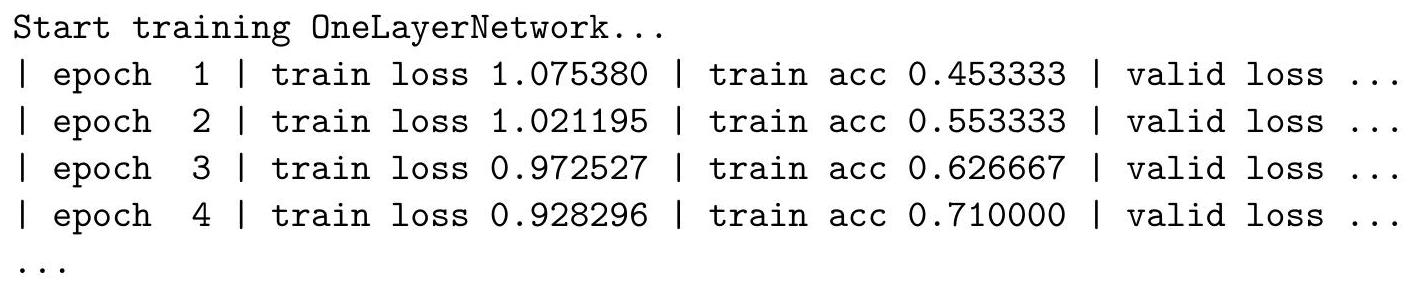
\includegraphics[max width=\textwidth]{2024_02_27_2131df32af4f1644e3f0g-3}
\end{center}

\section*{Two-Layer Network $[7 \mathrm{pts}]$}
For two-layer network, we consider a 784-400-3 network. In other words, the first layer will consist of a fully connected layer with $784 \times 400$ weight matrix $\mathbf{W}_{1}$ and a second layer consisting of $400 \times 3$ weight matrix $\mathbf{W}_{2}$. Given a $\mathbf{x}_{n}$, we can compute the probability vector $\mathbf{p}_{n}=$ $\operatorname{Softmax}\left(\mathbf{W}_{2}^{\top} \sigma\left(\mathbf{W}_{1}^{\top} \mathbf{x}_{n}\right)\right)$, where $\sigma($.$) is the element-wise sigmoid function. Again, we focus on the$ cross entropy loss, hence the network will implement $\mathbf{W}_{2}^{\top} \sigma\left(\mathbf{W}_{1}^{\top} \mathbf{x}_{n}\right)$ (note the softmax will be taken care of implicitly in our loss). The bias term is included in torch.nn.Linear by default, do not disable that option.

\section*{Solution 3f:}

\begin{minted}{python}
            ### ========== TODO : START ========== ###
            ### part f: implement the training process
            #pass
            y_pred = model.forward(batch_X)
            model.zero_grad()
            loss = criterion(y_pred, batch_y)
            loss.backward()
            optimizer.step()
            ### ========== TODO : END ========== ###
\end{minted}

(g) (5 pts) Implement the constructor of TwoLayerNetwork with torch.nn.Linear and implement the forward function to compute $\mathbf{W}_{2}^{\top} \sigma\left(\mathbf{W}_{1}^{\top} \mathbf{x}_{n}\right)$.

\section*{Solution 3g:}

\begin{minted}{python}
class TwoLayerNetwork(torch.nn.Module):
    def __init__(self):
        super(TwoLayerNetwork, self).__init__()
        ### ========== TODO : START ========== ###
        ### part g: implement TwoLayerNetwork with torch.nn.Linear
        self.hidden_layer = torch.nn.Linear(784, 400)
        self.output_layer = torch.nn.Linear(400, 3)
        ### ========== TODO : END ========== ###

    def forward(self, x):
        # x.shape = (n_batch, n_features)

        ### ========== TODO : START ========== ###
        ### part g: implement the foward function
        sigmoid = torch.nn.Sigmoid()
        layer = self.hidden_layer(x)
        layer = sigmoid(layer)
        outputs = self.output_layer(layer)
        ### ========== TODO : END ========== ###
        return outputs
\end{minted}

(h) (2 pts) Create an instance of TwoLayerNetwork, set up a criterion with torch.nn. CrossEntropyLoss, and set up a SGD optimizer with learning rate 0.0005 by using torch.optim. SGD. Then train TwoLayerNetwork.

\section*{Solution 3h:}

\begin{minted}{python}
    ### ========== TODO : START ========== ###
    ### part h: prepare TwoLayerNetwork, criterion, and optimizer
    model_two = TwoLayerNetwork()
    criterion = torch.nn.CrossEntropyLoss()
    optimizer = torch.optim.SGD(model_two.parameters(), lr=0.0005)
    ### ========== TODO : END ========== ###
\end{minted}

\section*{Performance Comparison [16 pts]}
(i) (3 pts) Generate a plot depicting how one\_train\_loss, one\_valid\_loss, two\_train\_loss, two\_valid\_loss varies with epochs. Include the plot in the report and describe your findings.

\section*{Solution 3i:}

\begin{minted}[breaklines]{python}
    ### ========== TODO : START ========== ###
    ### part i: generate a plot to comare one_train_loss, one_valid_loss, two_train_loss, two_valid_loss
    epochs = np.arange(1, 31)
    plt.figure(figsize=[10,10])
    plt.plot(epochs, one_train_loss, color='yellow', label='One Layer Training Loss', marker='x')
    plt.plot(epochs, one_valid_loss, color='blue', label='One Layer Validity Loss', marker='x')
    #Go Warriors! >:)
    plt.plot(epochs, two_train_loss, color='red', label='Two Layer Training Loss', marker='x')
    plt.plot(epochs, two_valid_loss, color='gold', label='Two Layer Validity Loss', marker='x')
    #Go Niners! >:), but we loss :(
    plt.xlabel('Epochs')
    plt.ylabel('Loss')
    plt.title('Epochs vs Loss (Training and Validity Loss)')
    plt.legend()
    plt.show()
    ### ========== TODO : END ========== ###
\end{minted}

\begin{figure}
    \centering
    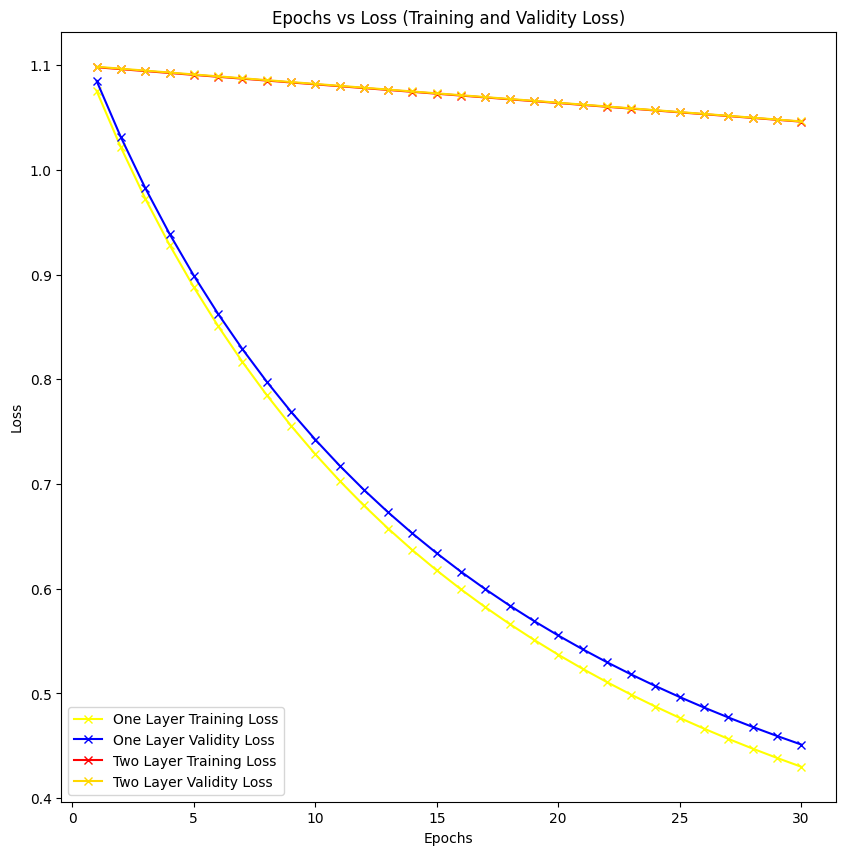
\includegraphics[width= 10cm, height = 10cm]{images/4i.png}
    \caption{Epoch vs Loss}
    \label{fig:enter-label}
\end{figure}

The reduction in loss for both the training and validation sets progresses at a slower pace in the model with two layers when compared to the model with a single layer. This slower progression of learning in the two-layered model is attributed to the process of back-propagation of the error gradient through the network, which involves making adjustments based on the chain rule. This can lead to the generation of very small derivatives, resulting in minimal changes to the weights of the initial layers during adjustments. Conversely, the network with one layer contains fewer parameters, facilitating easier optimization and enabling faster achievement of convergence. Moreover, the similarity in training and validation loss between both models suggests effective generalization without the presence of overfitting. \\

(j) (3 pts) Generate a plot depicting how one\_train\_acc, one\_valid\_acc, two\_train\_acc, two\_valid\_acc varies with epochs. Include the plot in the report and describe your findings.

\section*{Solution 3j:}

\begin{minted}[breaklines]{python}
    ### ========== TODO : START ========== ###
    ### part j: generate a plot to comare one_train_acc, one_valid_acc, two_train_acc, two_valid_acc
    epochs = np.arange(1, 31)
    plt.figure(figsize=[10,10])
    plt.plot(epochs, one_train_acc, color='yellow', label='One Layer Training Accuracy', marker='x')
    plt.plot(epochs, one_valid_acc, color='blue', label='One Layer Validity Accuracy', marker='x')
    #Go Warriors! >:)
    plt.plot(epochs, two_train_acc, color='red', label='Two Layer Training Accuracy', marker='x')
    plt.plot(epochs, two_valid_acc, color='gold', label='Two Layer Validity Accuracy', marker='x')
    #Go Niners! >:), but we loss :(
    plt.xlabel('Epochs')
    plt.ylabel('Accuracy')
    plt.title('Epochs vs Accuracy (Training and Validity Accuracy)')
    plt.legend()
    plt.show()
    ### ========== TODO : END ========== ##
\end{minted}

\begin{figure}[h!]
    \centering
    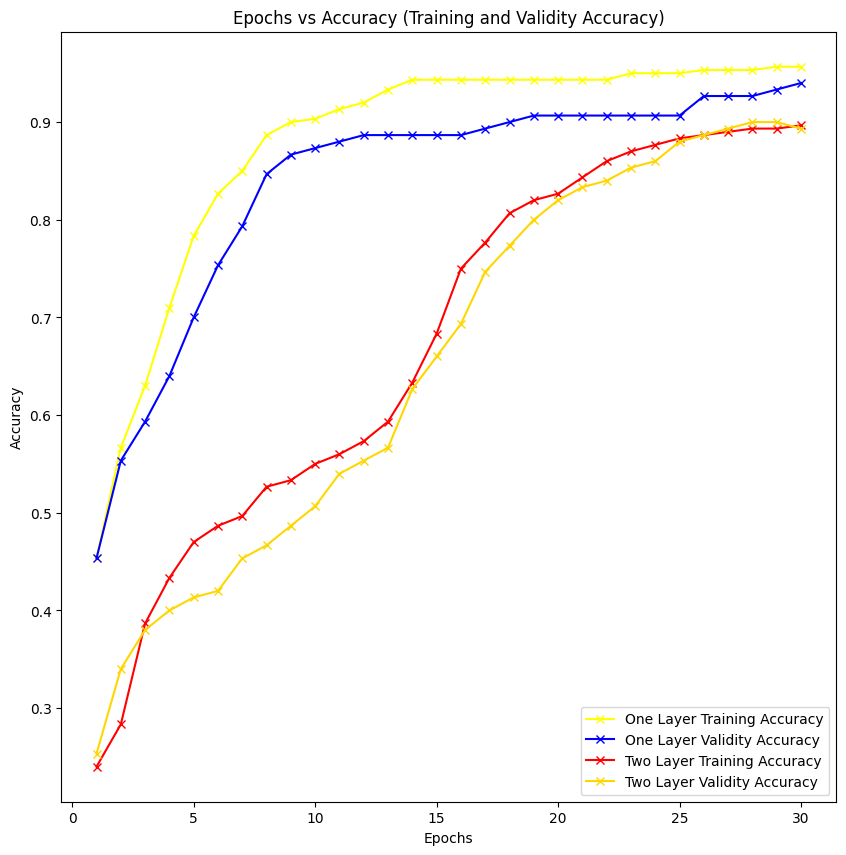
\includegraphics[width= 10cm, height = 10cm]{images/4j.png}
    \caption{Epoch vs Accuracy}
    \label{fig:enter-label}
\end{figure} 

The chart shows that the neural network with a single layer outperforms the neural network with two layers in terms of reaching convergence more efficiently. The slower increase in precision for the two-layered network can be attributed to its larger number of weights and the complexities involved in back-propagating through these weights, leading to minor derivatives and consequently slow weight adjustments. Nevertheless, the accuracy levels of both networks tend to align more closely in the later stages of training. It's also observed that the accuracy on the validation dataset consistently trails behind the training dataset accuracy, suggesting a slight risk of over-fitting. Yet, the models demonstrate good generalization capabilities as the discrepancy is relatively small. The neural network with a single layer achieves training and validation accuracies around 96 percent, whereas the two-layer network reaches training and validation accuracies about 90 percent. \\

(k) (3 pts) Calculate and report the test accuracy of both the one-layer network and the two-layer network. How can you improve the performance of the two-layer network?

\section*{Solution 3k:}

\begin{minted}[breaklines]{python}
    ### ========== TODO : START ========== ###
    ### part k: calculate the test accuracy
    print("One Layer Network Test Accuracy: ", evaluate_acc(model_one, test_loader))
    print("Two Layer Network Test Accuracy: ", evaluate_acc(model_two, test_loader))
    ### ========== TODO : END ========== ###
\end{minted}

How to Improve: \\
The accuracy of the single-layer network significantly surpasses that of the dual-layer network, which might be explained by two key factors. First, the increased number of parameters in the two-layer network could necessitate a more extended training duration beyond the 30 epochs used in the experiment. Second, there's a chance the two-layer network experienced overfitting, although the accuracy versus epoch chart indicates that, if this occurred, its impact is minimal. \\


Results: \\
One Layer Network Test Accuracy:  tensor(0.9600) \\
Two Layer Network Test Accuracy:  tensor(0.9000) \\

(1) (7 pts) Replace the SGD optimizer with the Adam optimizer and do the experiments again. Show the loss figure, the accuracy figure, and the test accuracy. Include the figures in the report and describe your findings.

You can refer to \href{https://pytorch.org/docs/stable/optim.html}{https://pytorch.org/docs/stable/optim.html} for more information about torch.optim. Adam.

\section*{Solution 3l:}

SGD Epochs:
\begin{minted}[breaklines]{text}
Start training OneLayerNetwork...
| epoch  1 | train loss 1.075398 | train acc 0.453333 | valid loss 1.084938 | valid acc 0.453333 |
| epoch  2 | train loss 1.021364 | train acc 0.566667 | valid loss 1.031102 | valid acc 0.553333 |
| epoch  3 | train loss 0.972648 | train acc 0.630000 | valid loss 0.982742 | valid acc 0.593333 |
| epoch  4 | train loss 0.928398 | train acc 0.710000 | valid loss 0.938953 | valid acc 0.640000 |
| epoch  5 | train loss 0.887963 | train acc 0.783333 | valid loss 0.899045 | valid acc 0.700000 |
| epoch  6 | train loss 0.850839 | train acc 0.826667 | valid loss 0.862485 | valid acc 0.753333 |
| epoch  7 | train loss 0.816627 | train acc 0.850000 | valid loss 0.828852 | valid acc 0.793333 |
| epoch  8 | train loss 0.785000 | train acc 0.886667 | valid loss 0.797807 | valid acc 0.846667 |
| epoch  9 | train loss 0.755688 | train acc 0.900000 | valid loss 0.769067 | valid acc 0.866667 |
| epoch 10 | train loss 0.728461 | train acc 0.903333 | valid loss 0.742397 | valid acc 0.873333 |
| epoch 11 | train loss 0.703122 | train acc 0.913333 | valid loss 0.717596 | valid acc 0.880000 |
| epoch 12 | train loss 0.679499 | train acc 0.920000 | valid loss 0.694488 | valid acc 0.886667 |
| epoch 13 | train loss 0.657439 | train acc 0.933333 | valid loss 0.672921 | valid acc 0.886667 |
| epoch 14 | train loss 0.636807 | train acc 0.943333 | valid loss 0.652760 | valid acc 0.886667 |
| epoch 15 | train loss 0.617482 | train acc 0.943333 | valid loss 0.633883 | valid acc 0.886667 |
| epoch 16 | train loss 0.599356 | train acc 0.943333 | valid loss 0.616184 | valid acc 0.886667 |
| epoch 17 | train loss 0.582330 | train acc 0.943333 | valid loss 0.599565 | valid acc 0.893333 |
| epoch 18 | train loss 0.566316 | train acc 0.943333 | valid loss 0.583938 | valid acc 0.900000 |
| epoch 19 | train loss 0.551234 | train acc 0.943333 | valid loss 0.569225 | valid acc 0.906667 |
| epoch 20 | train loss 0.537010 | train acc 0.943333 | valid loss 0.555355 | valid acc 0.906667 |
| epoch 21 | train loss 0.523580 | train acc 0.943333 | valid loss 0.542262 | valid acc 0.906667 |
| epoch 22 | train loss 0.510882 | train acc 0.943333 | valid loss 0.529888 | valid acc 0.906667 |
| epoch 23 | train loss 0.498862 | train acc 0.950000 | valid loss 0.518179 | valid acc 0.906667 |
| epoch 24 | train loss 0.487470 | train acc 0.950000 | valid loss 0.507086 | valid acc 0.906667 |
| epoch 25 | train loss 0.476660 | train acc 0.950000 | valid loss 0.496564 | valid acc 0.906667 |
| epoch 26 | train loss 0.466391 | train acc 0.953333 | valid loss 0.486573 | valid acc 0.926667 |
| epoch 27 | train loss 0.456625 | train acc 0.953333 | valid loss 0.477076 | valid acc 0.926667 |
| epoch 28 | train loss 0.447328 | train acc 0.953333 | valid loss 0.468038 | valid acc 0.926667 |
| epoch 29 | train loss 0.438467 | train acc 0.956667 | valid loss 0.459429 | valid acc 0.933333 |
| epoch 30 | train loss 0.430013 | train acc 0.956667 | valid loss 0.451220 | valid acc 0.940000 |
Done!
Start training TwoLayerNetwork...
| epoch  1 | train loss 1.098020 | train acc 0.240000 | valid loss 1.098498 | valid acc 0.253333 |
| epoch  2 | train loss 1.096157 | train acc 0.283333 | valid loss 1.096622 | valid acc 0.340000 |
| epoch  3 | train loss 1.094329 | train acc 0.386667 | valid loss 1.094783 | valid acc 0.380000 |
| epoch  4 | train loss 1.092512 | train acc 0.433333 | valid loss 1.092956 | valid acc 0.400000 |
| epoch  5 | train loss 1.090700 | train acc 0.470000 | valid loss 1.091135 | valid acc 0.413333 |
| epoch  6 | train loss 1.088891 | train acc 0.486667 | valid loss 1.089318 | valid acc 0.420000 |
| epoch  7 | train loss 1.087085 | train acc 0.496667 | valid loss 1.087503 | valid acc 0.453333 |
| epoch  8 | train loss 1.085281 | train acc 0.526667 | valid loss 1.085691 | valid acc 0.466667 |
| epoch  9 | train loss 1.083480 | train acc 0.533333 | valid loss 1.083882 | valid acc 0.486667 |
| epoch 10 | train loss 1.081682 | train acc 0.550000 | valid loss 1.082076 | valid acc 0.506667 |
| epoch 11 | train loss 1.079886 | train acc 0.560000 | valid loss 1.080273 | valid acc 0.540000 |
| epoch 12 | train loss 1.078093 | train acc 0.573333 | valid loss 1.078472 | valid acc 0.553333 |
| epoch 13 | train loss 1.076302 | train acc 0.593333 | valid loss 1.076674 | valid acc 0.566667 |
| epoch 14 | train loss 1.074514 | train acc 0.633333 | valid loss 1.074878 | valid acc 0.626667 |
| epoch 15 | train loss 1.072727 | train acc 0.683333 | valid loss 1.073084 | valid acc 0.660000 |
| epoch 16 | train loss 1.070942 | train acc 0.750000 | valid loss 1.071292 | valid acc 0.693333 |
| epoch 17 | train loss 1.069159 | train acc 0.776667 | valid loss 1.069502 | valid acc 0.746667 |
| epoch 18 | train loss 1.067377 | train acc 0.806667 | valid loss 1.067713 | valid acc 0.773333 |
| epoch 19 | train loss 1.065597 | train acc 0.820000 | valid loss 1.065926 | valid acc 0.800000 |
| epoch 20 | train loss 1.063817 | train acc 0.826667 | valid loss 1.064139 | valid acc 0.820000 |
| epoch 21 | train loss 1.062038 | train acc 0.843333 | valid loss 1.062354 | valid acc 0.833333 |
| epoch 22 | train loss 1.060260 | train acc 0.860000 | valid loss 1.060569 | valid acc 0.840000 |
| epoch 23 | train loss 1.058483 | train acc 0.870000 | valid loss 1.058785 | valid acc 0.853333 |
| epoch 24 | train loss 1.056706 | train acc 0.876667 | valid loss 1.057001 | valid acc 0.860000 |
| epoch 25 | train loss 1.054928 | train acc 0.883333 | valid loss 1.055217 | valid acc 0.880000 |
| epoch 26 | train loss 1.053151 | train acc 0.886667 | valid loss 1.053433 | valid acc 0.886667 |
| epoch 27 | train loss 1.051374 | train acc 0.890000 | valid loss 1.051650 | valid acc 0.893333 |
| epoch 28 | train loss 1.049596 | train acc 0.893333 | valid loss 1.049865 | valid acc 0.900000 |
| epoch 29 | train loss 1.047818 | train acc 0.893333 | valid loss 1.048081 | valid acc 0.900000 |
| epoch 30 | train loss 1.046038 | train acc 0.896667 | valid loss 1.046295 | valid acc 0.893333 |
Done!
\end{minted}

Adam Epochs:
\begin{minted}[breaklines]{text}
Start training OneLayerNetwork...
| epoch  1 | train loss 0.652176 | train acc 0.930000 | valid loss 0.643495 | valid acc 0.900000 |
| epoch  2 | train loss 0.448845 | train acc 0.960000 | valid loss 0.450156 | valid acc 0.953333 |
| epoch  3 | train loss 0.340191 | train acc 0.970000 | valid loss 0.347157 | valid acc 0.953333 |
| epoch  4 | train loss 0.275654 | train acc 0.976667 | valid loss 0.286565 | valid acc 0.953333 |
| epoch  5 | train loss 0.233069 | train acc 0.976667 | valid loss 0.247042 | valid acc 0.953333 |
| epoch  6 | train loss 0.202674 | train acc 0.976667 | valid loss 0.219164 | valid acc 0.960000 |
| epoch  7 | train loss 0.179708 | train acc 0.976667 | valid loss 0.198359 | valid acc 0.960000 |
| epoch  8 | train loss 0.161607 | train acc 0.980000 | valid loss 0.182174 | valid acc 0.960000 |
| epoch  9 | train loss 0.146879 | train acc 0.980000 | valid loss 0.169180 | valid acc 0.966667 |
| epoch 10 | train loss 0.134596 | train acc 0.980000 | valid loss 0.158487 | valid acc 0.973333 |
| epoch 11 | train loss 0.124151 | train acc 0.983333 | valid loss 0.149514 | valid acc 0.973333 |
| epoch 12 | train loss 0.115131 | train acc 0.986667 | valid loss 0.141863 | valid acc 0.980000 |
| epoch 13 | train loss 0.107242 | train acc 0.986667 | valid loss 0.135252 | valid acc 0.980000 |
| epoch 14 | train loss 0.100269 | train acc 0.986667 | valid loss 0.129476 | valid acc 0.980000 |
| epoch 15 | train loss 0.094054 | train acc 0.990000 | valid loss 0.124380 | valid acc 0.980000 |
| epoch 16 | train loss 0.088473 | train acc 0.990000 | valid loss 0.119847 | valid acc 0.980000 |
| epoch 17 | train loss 0.083429 | train acc 0.990000 | valid loss 0.115785 | valid acc 0.980000 |
| epoch 18 | train loss 0.078848 | train acc 0.990000 | valid loss 0.112121 | valid acc 0.980000 |
| epoch 19 | train loss 0.074666 | train acc 0.990000 | valid loss 0.108797 | valid acc 0.980000 |
| epoch 20 | train loss 0.070834 | train acc 0.990000 | valid loss 0.105767 | valid acc 0.980000 |
| epoch 21 | train loss 0.067309 | train acc 0.990000 | valid loss 0.102990 | valid acc 0.980000 |
| epoch 22 | train loss 0.064057 | train acc 0.990000 | valid loss 0.100436 | valid acc 0.980000 |
| epoch 23 | train loss 0.061046 | train acc 0.993333 | valid loss 0.098077 | valid acc 0.980000 |
| epoch 24 | train loss 0.058253 | train acc 0.993333 | valid loss 0.095891 | valid acc 0.980000 |
| epoch 25 | train loss 0.055655 | train acc 0.993333 | valid loss 0.093858 | valid acc 0.980000 |
| epoch 26 | train loss 0.053232 | train acc 0.996667 | valid loss 0.091962 | valid acc 0.980000 |
| epoch 27 | train loss 0.050969 | train acc 0.996667 | valid loss 0.090190 | valid acc 0.980000 |
| epoch 28 | train loss 0.048851 | train acc 1.000000 | valid loss 0.088529 | valid acc 0.980000 |
| epoch 29 | train loss 0.046865 | train acc 1.000000 | valid loss 0.086968 | valid acc 0.980000 |
| epoch 30 | train loss 0.045000 | train acc 1.000000 | valid loss 0.085498 | valid acc 0.980000 |
Done!
Start training TwoLayerNetwork...
| epoch  1 | train loss 0.493845 | train acc 0.963333 | valid loss 0.499119 | valid acc 0.946667 |
| epoch  2 | train loss 0.268077 | train acc 0.980000 | valid loss 0.286093 | valid acc 0.960000 |
| epoch  3 | train loss 0.171713 | train acc 0.983333 | valid loss 0.199556 | valid acc 0.960000 |
| epoch  4 | train loss 0.122286 | train acc 0.983333 | valid loss 0.156994 | valid acc 0.966667 |
| epoch  5 | train loss 0.093136 | train acc 0.986667 | valid loss 0.133069 | valid acc 0.966667 |
| epoch  6 | train loss 0.073462 | train acc 0.993333 | valid loss 0.117480 | valid acc 0.966667 |
| epoch  7 | train loss 0.059191 | train acc 0.996667 | valid loss 0.106445 | valid acc 0.966667 |
| epoch  8 | train loss 0.048472 | train acc 1.000000 | valid loss 0.098250 | valid acc 0.973333 |
| epoch  9 | train loss 0.040236 | train acc 1.000000 | valid loss 0.091944 | valid acc 0.973333 |
| epoch 10 | train loss 0.033800 | train acc 1.000000 | valid loss 0.086957 | valid acc 0.973333 |
| epoch 11 | train loss 0.028701 | train acc 1.000000 | valid loss 0.082925 | valid acc 0.973333 |
| epoch 12 | train loss 0.024610 | train acc 1.000000 | valid loss 0.079609 | valid acc 0.973333 |
| epoch 13 | train loss 0.021291 | train acc 1.000000 | valid loss 0.076844 | valid acc 0.973333 |
| epoch 14 | train loss 0.018572 | train acc 1.000000 | valid loss 0.074512 | valid acc 0.980000 |
| epoch 15 | train loss 0.016322 | train acc 1.000000 | valid loss 0.072525 | valid acc 0.980000 |
| epoch 16 | train loss 0.014443 | train acc 1.000000 | valid loss 0.070818 | valid acc 0.980000 |
| epoch 17 | train loss 0.012861 | train acc 1.000000 | valid loss 0.069341 | valid acc 0.980000 |
| epoch 18 | train loss 0.011519 | train acc 1.000000 | valid loss 0.068053 | valid acc 0.980000 |
| epoch 19 | train loss 0.010371 | train acc 1.000000 | valid loss 0.066924 | valid acc 0.980000 |
| epoch 20 | train loss 0.009382 | train acc 1.000000 | valid loss 0.065928 | valid acc 0.980000 |
| epoch 21 | train loss 0.008525 | train acc 1.000000 | valid loss 0.065045 | valid acc 0.980000 |
| epoch 22 | train loss 0.007778 | train acc 1.000000 | valid loss 0.064258 | valid acc 0.980000 |
| epoch 23 | train loss 0.007123 | train acc 1.000000 | valid loss 0.063554 | valid acc 0.980000 |
| epoch 24 | train loss 0.006546 | train acc 1.000000 | valid loss 0.062922 | valid acc 0.980000 |
| epoch 25 | train loss 0.006035 | train acc 1.000000 | valid loss 0.062352 | valid acc 0.980000 |
| epoch 26 | train loss 0.005581 | train acc 1.000000 | valid loss 0.061836 | valid acc 0.980000 |
| epoch 27 | train loss 0.005174 | train acc 1.000000 | valid loss 0.061368 | valid acc 0.980000 |
| epoch 28 | train loss 0.004810 | train acc 1.000000 | valid loss 0.060942 | valid acc 0.980000 |
| epoch 29 | train loss 0.004482 | train acc 1.000000 | valid loss 0.060553 | valid acc 0.980000 |
| epoch 30 | train loss 0.004186 | train acc 1.000000 | valid loss 0.060198 | valid acc 0.980000 |
Done!
\end{minted}

The Adam optimizer leads to faster convergence compared to the SGD optimizer, allowing the two-layer network's true accuracy to be realized as it converges. The data from the graphs show that the two-layer network outperforms the one-layer network in both training and validation datasets, while performing equally on the test dataset. Within just five epochs, the two-layer network reaches a validation accuracy of 97.5 percent. The reason behind the similar test accuracies for both models could be attributed to the constraints of a small dataset. Learning theory suggests that generalization error is influenced by the size of the training dataset, and anomalies in the test dataset might hinder achieving a 100 percent accuracy. Thus, it could be that both models have extracted as much as possible from the limited training data available, leading to identical or similar test accuracy outcomes. For us it was 97.33 percent and 96.67 percent respectively. \\

Results:\\
One Layer Network Test Accuracy:  tensor(0.9733)\\
Two Layer Network Test Accuracy:  tensor(0.9667)\\

\begin{figure}[ht]
    \centering
    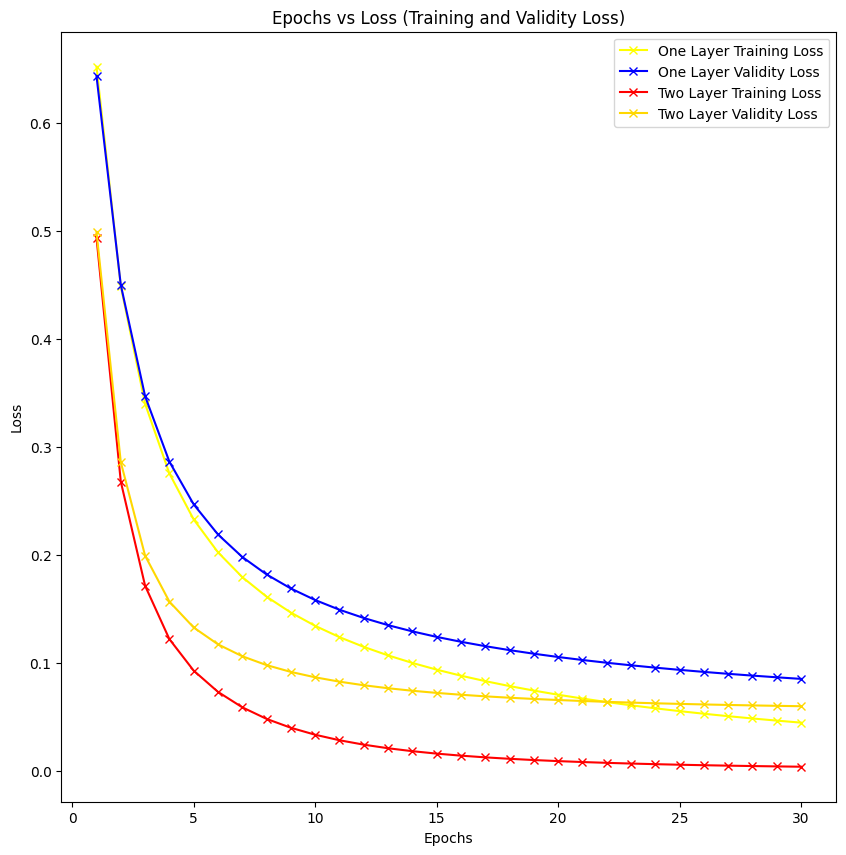
\includegraphics[width= 10cm, height = 10cm]{images/4l_1.png}
    \caption{Epoch vs Loss (Adam)}
    \label{fig:enter-label}
\end{figure} 

\begin{figure}[ht]
    \centering
    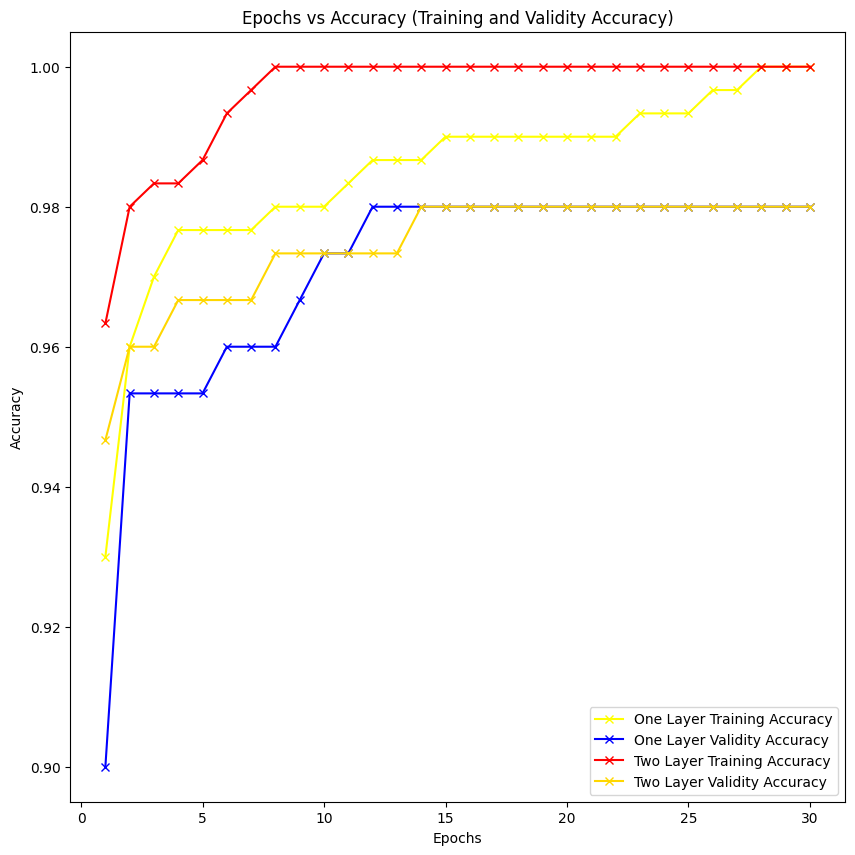
\includegraphics[width= 10cm, height = 10cm]{images/4l_2.png}
    \caption{Epoch vs Accuracy (Adam)}
    \label{fig:enter-label}
\end{figure} 


\end{document}